\subsection{System Context}
\progname{}'s system context includes: the user; a development
environment---which might not be specialized for game development---where users
define at least one game entity associated with one or more \progname{}
instance and any number of game entities that are not associated with an
instance of \progname{}; and the game environment containing the game entities
defined in the development environment. Figure~\ref{fig_sysContext} visually
describes this, with the human user represented by a circle, game entities by
``cards'', and software systems by rectangles. Game entities and software
systems are collected into ``environments'', represented by containers.
Enumerated associations between elements are defined with Unified Modelling
Language (UML) relationships.

\begin{figure}[!ht]
    \centering
    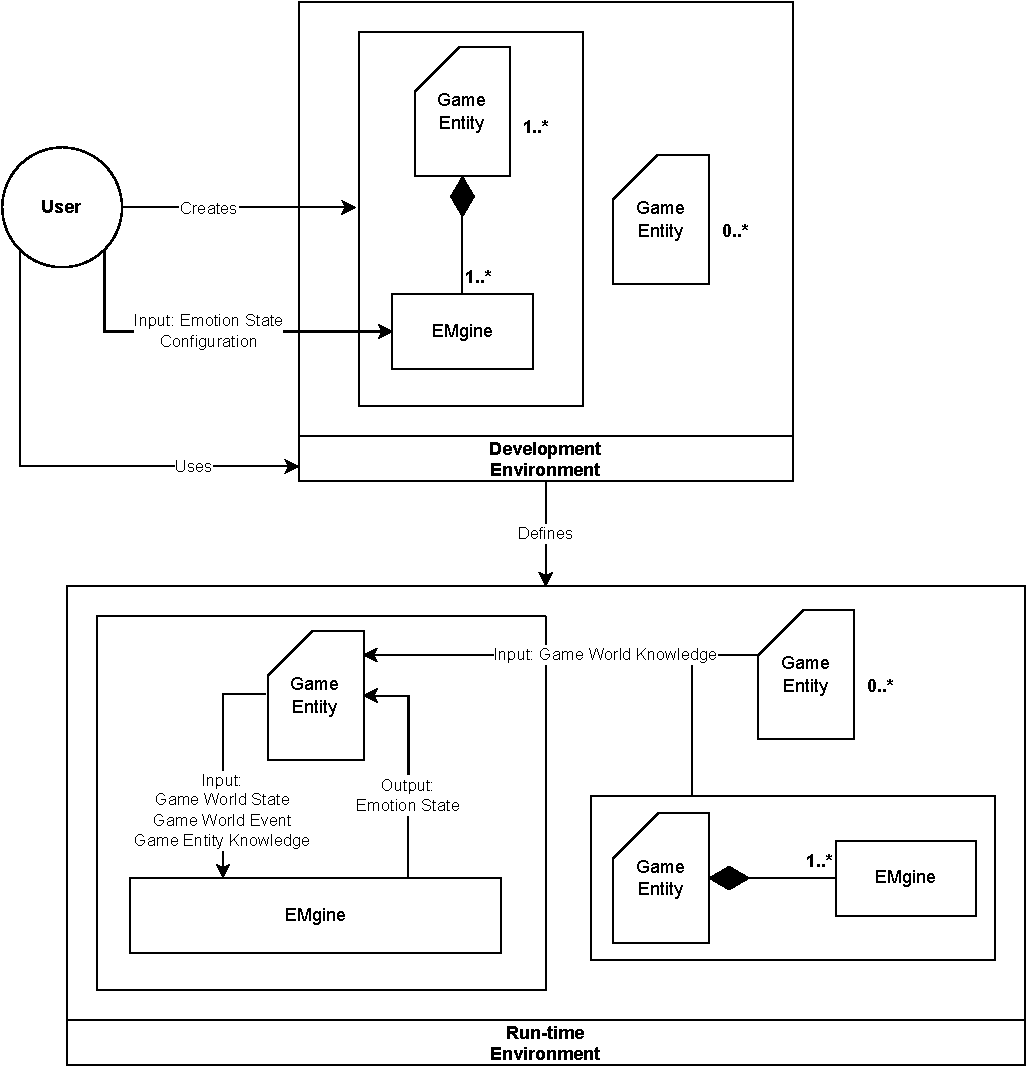
\includegraphics[width=0.9\textwidth]{figures/systemContext_Revised.pdf}
    \caption{System Context}
    \label{fig_sysContext}
\end{figure}

Within this context, each element has responsibilities to ensure that
\progname{} can function correctly:
\begin{enumerate}

    \item User (Game Designer/Developer) Responsibilities
    \begin{itemize}
        \item Associate at least one game entity with one or more \progname{}
        instances
        \item Provide functions required to evaluate \progname{}'s
        time-dependent inputs
        \item Associate \progname{} emotion types with game entity animations,
        audio, and/or behaviours
    \end{itemize}

    \item Development Environment Responsibilities
    \begin{itemize}
        \item Provide a method for interfacing with third-party systems
    \end{itemize}

    \item Run-time Environment Responsibilities
    \begin{itemize}
        \item Allow game entities to store and/or update information
        \item Allow game entities to exchange information
    \end{itemize}

    \item Game Entity Responsibilities
    \begin{itemize}
        \item Send information about events and objects in the game environment
        to one or more of their associated \progname{} instances
        \item Execute animations, audio and/or behaviours associated with
        \progname{} emotion types based on its outputs
    \end{itemize}

    \item \progname{} Responsibilities
    \begin{itemize}
        \item Detect and prevent data type mismatch, such as a string of
        characters instead of a floating point number
        \item Allow users to modify its default parameters
        \item Allow users to define new emotion types
        \item Evaluate incoming information and make corresponding updates to
        its emotion state
        \item Allow game entities to query its emotion state
    \end{itemize}

\end{enumerate}